\section{Filtro 2: Merge}

\subsection{Explicacion}
El filtro $merge$ consiste en tomar 2 imagenes del mismo tamaño y un parametro (llamdo \texttt{value} en el enunciado) de tipo $float$ entre 0 y 1, multiplicar las componetes de la primer imagen por \texttt{value} y los de la segunda por \texttt{1 - value} y sumar los pixeles de ambas para crear una nueva imagen. \\

\subsection{Implementacion 1}
Para la primer implementacion se nos pidio trabajar con valores de tipo $float$, procesando la mayor cantidad de pixeles posibles por iteracion. \\

Ya que la cantidad de pixeles por imagen siempre va a ser un multiplo de 4 segun el enunciado, decidimos tomar de a 4 pixeles de la memoria para trabajar con los mismos, esto nos permitio simplificar el ciclo y operar sin tener que preocuparnos por excedernos del area de memoria alocada a la imagen.\\

Para procesar los pixeles del merge utilizamos 2 registros \texttt{XMM} para guardar los 4 pixeles como bytes que obtenemos de la memoria, y 2 registros mas para guardar copias de los mismos. Ademas como utilizamos una funcion auxiliar tambien precisamos de 4 registros \texttt{XMM} mas para poder guardar los resultados de la funcion. Por ultimo, tenemos \texttt{value} y \texttt{1 - value} guardados en los registros \texttt{XMM15} y \texttt{XMM14} respectivamente. Ademas de estos registros, se emplearon tambien los siguientes de proposito general:\\

\noindent
\begin{itemize}
	\item \texttt{RDX} puntero a la primera imagen
	\item \texttt{RCD} puntero a la segunda imagen
	\item \texttt{R9} iterador en \texttt{Y}
	\item \texttt{R8} iterador en \texttt{X}
\end{itemize}

Esta distribucion de registros reponde al siguiente grafico:

\begin{figure}[h!]
	\centering
	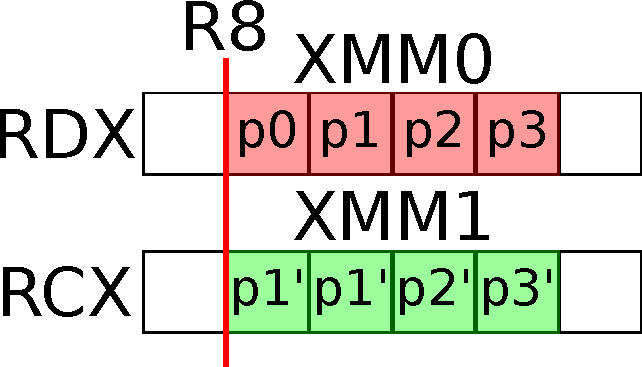
\includegraphics[scale=0.5]{images/MergeASM1_0}
\end{figure}

Antes de empezar a recorrer la imagen, para asignar los valores correctos de \texttt{XMM14} y \texttt{XMM15} utilizamos el dato \texttt{value} original almacenado en \texttt{XMM0}. Este valor fue copiado mediante un operacion de shuffle hacia \texttt{XMM15}, esta operacion copiaba \texttt{value} a todas las componentes de \texttt{XMM15}. Para poder calcular \texttt{XMM14} alcanzo con mover al mismo una constante almacenada en memoria que tuviese \texttt{1.0} en los 4 $float$ y posteriormente restarle el contenido de \texttt{XMM15}. Finalmente tenemos en \texttt{XMM14} y \texttt{XMM15}:\\

\noindent
\texttt{XMM14 $\gets$ 1 - value $\vert$ 1 - value $\vert$ 1 - value $\vert$ 1 - value}\\
\texttt{XMM15 $\gets\ \ $ value $\ \ \vert\ \ $ value $\ \ \vert\ \ $ value $\ \ \vert\ \ $ value}\\

Para poder movernos por la imagen empleamos dos ciclos anidados, el primero de ellos nos permite, junto con \texttt{R9}, iterar sobre el eje \texttt{Y}, mientras que el ciclo interno nos permite movernos con facilidad sobre el eje \texttt{X} mediante \texttt{R8}. Antes de comenzar a iterar en el ciclo principal, incializamos ambos iteradores en 0, y si llegamos al final del ciclo interno (es decir, iteramos sobre todo el eje \texttt{X} para la fila actual) colocamos el iterador de \texttt{X} en 0. Al comienzo de cada ciclo de \texttt{X}, movemos hacia los registros \texttt{XMM0} y \texttt{XMM1} los datos de los pixeles a procesar de la primer y segunda imagen respectivamente, ademas copiamos cada una en \texttt{XMM2} y \texttt{XMM3}, luego de esto procedimos a llamar a la funcion auxiliar \texttt{addPixels} 4 veces. Al finalizar los llamados, tenemos en \texttt{XMM4} los 4 pixeles procesados, lo unico restante fue volcarlos en memoria. Una vez que los pixeles se encuentran en memoria, tenemos que aumentar el iterador de \texttt{X} en 16 bytes, y en caso de haber llegado al final de la fila, colocar el mismo en 0 e incrementar el de \texttt{Y}. Si ya llegue al final de la imagen, termino el ciclo principal de la implementacion y procedo a retornar de la funcion.

La funcion \texttt{addPixels} es una funcion auxiliar la cual hace la aritmetica necesaria para poder mergear las imagenes, esta funcion toma los valores de \texttt{XMM2} y \texttt{XMM3} y los copia hacia \texttt{XMM0} y \texttt{XMM1} respectivamente, luego procede a desempaquetarlos a doubleword utilizando el registro \texttt{XMM10} el cual contiene 0 en todas sus componentes. Una vez desempaquetados los valores, se procede a convertirlos a tipo $float$ para poder realizar el producto con \texttt{XMM14} (\texttt{1-value}) y \texttt{XMM15} (\texttt{value}). Entonces tenemos:

\noindent
\texttt{XMM0 $\gets$ a * value $\vert$ r * value $\vert$ g * value $\vert$ b * value}
\texttt{XMM1 $\gets$ a * (1 - value) $\vert$ r * (1 - value) $\vert$ g * (1 - value) $\vert$ b * (1 - value)}

Con estos valores en los registros, lo unico restante es sumarlos, convertirlos nuevamente a entero, y empaquetarlos a byte. Antes de finalizar la funcion, shifteamos los registros \texttt{XMM2} y \texttt{XMM3} 4 bytes a la derecha, asi en el siguiente llamado a la funcion ya van a estar los siguientes pixeles a procesar en el lugar correcto.

\subsection{Implementacion 2}
Para la segunda implementacion se no pidio trabajar con enteros procesando la mayor cantidad de enteros posibles por iteracion. Al igual que en la primera implementacion trabajamos de a 4 pixeles al mismo tiempo por que nos permite iterar de manera segura. Al igual que antes vamos a emplear los registros \texttt{XMM14} y \texttt{XMM15} para guardar los valores por los cuales vamos a multiplicar los pixeles. Para calcularlos movimos \texttt{value} a XMM15, luego aplicamos un shuffle para que los 4 floats de \texttt{XMM15} \texttt{value}, luego movimos a \texttt{XMM14} una constante de $float$ almacenada en memoria la cual contenia \texttt{8192.0} en cada una de sus componentes, este registro fue multiplicado por \texttt{XMM15} almacenando el resultado del producto en \texttt{XMM15}, para obtener el \texttt{1 - value} lo unico necesario fue restarle a \texttt{XMM14} el contenido de \texttt{XMM15}. Finalmente tenemos:\\

\noindent
\texttt{XMM15 $\gets$ 8192.0 * value $\vert$ 8192.0 * value $\vert$ 8192.0 * value $\vert$ 8192.0 * value}\\
\texttt{XMM14 $\gets$ 8192.0 - 8192.0 * value $\vert$ 8192.0 - 8192.0 * value $\vert$ 8192.0 - 8192.0 * value $\vert$ 8192.0 - 8192.0 * value}\\
\texttt{XMM14 $\gets$ 8192.0 *(1 - value) $\vert$ 8192.0 * (1 - value) $\vert$ 8192.0 * (1 - value) $\vert$ 8192.0 * (1 - value)}\\

El numero 8192, que es $2^{13}$ fue elegido de manera empirica, ya que era el numero mas pequeño que nos permitia que el margen de error fuese lo suficientemente pequeño para poder cumplir con el enunciado.

Ademas de estos registros vamos a emplear los mismos registros de proposito general que la primer implementacion, junto con los registros \texttt{XMM0} a \texttt{XMM7} para tomar los valores de la imagen de la memoria y desempaquetar.

\begin{figure}[h!]
	\centering
	\includegraphics[scale=0.5]{images/MergeASM2_0}
\end{figure}

La estructura de la primera implementacion se mantuvo igual, es decir, se preservo el ciclo anidado y el uso de iteradores, esto significa que las misma precauciones respecto a los mismos tomadas anteriormente aplican nuevamente en ese caso. Una vez dentro del ciclo de \texttt{X} procedimos a mover hacia \texttt{XMM0} y \texttt{XMM4} los grupos de pixeles de la primera y segunda imagen. Estos fueron desempaquetados a doubleword, quedando de la siguiente forma:

\noindent
\texttt{XMM0 $\gets$ p0}\\
\texttt{XMM1 $\gets$ p1}\\
\texttt{XMM2 $\gets$ p2}\\
\texttt{XMM3 $\gets$ p3}\\
\texttt{XMM4 $\gets$ p0'}\\
\texttt{XMM5 $\gets$ p1'}\\
\texttt{XMM6 $\gets$ p2'}\\
\texttt{XMM7 $\gets$ p3'}\\

Despues se multiplico a \texttt{XMM0}, \texttt{XMM1}, \texttt{XMM2} y \texttt{XMM3} por \texttt{XMM15}, el resultado de la operacion fue shifteado 14 bits hacia la derecha, obteniendo \texttt{(p * 8192 * v) / 8192 = p * v}. Esta misma logica se aplico con los otro cuatro registros, salvo que fueron multiplicados por \texttt{XMM14}, obteniendo \texttt{(p * 8192 * (1 - v) / 8192 = p * (1 - v)}. Una vez completado esto, finalmente tenemos cada pixel multiplicado por su \texttt{value} correspondiente, los mismos luego fueron empaquetados en un solo registro como muestra el grafico:

\begin{figure}[h!]
	\centering
	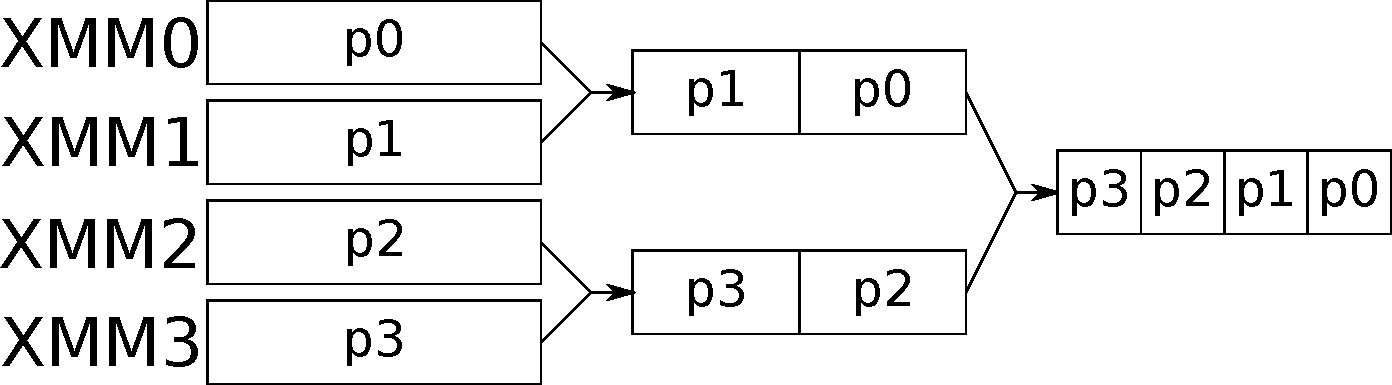
\includegraphics[scale=0.5]{images/MergeASM2_1}
\end{figure}

Al final tenemos:\\

\noindent
\texttt{XMM0 $\gets$ p3 * value $\vert$ p2 * value $\vert$ p1 * value $\vert$ p0 * value}\\
\texttt{XMM4 $\gets$ p3' * (1 - value) $\vert$ p2' * (1 - value) $\vert$ p1' * (1 - value) $\vert$ p0' * (1 - value)}\\

Para terminar solo fue necesario sumarlos y moverlos a memoria.

\subsection{Resultados}
Para la experimentacion vamos a correr las 3 implementaciones (La version de $C$ compilada con optimizaciones de nivel 3) con la imagen de $lena$ brindada por la catedra (multiplos de 16x16, hasta 320x320), se corren 100 veces cada tamaño y despues se saca un promedio y se grafica el maximo, el minimo y el promedio.

\begin{figure}[h!]
	\centering
	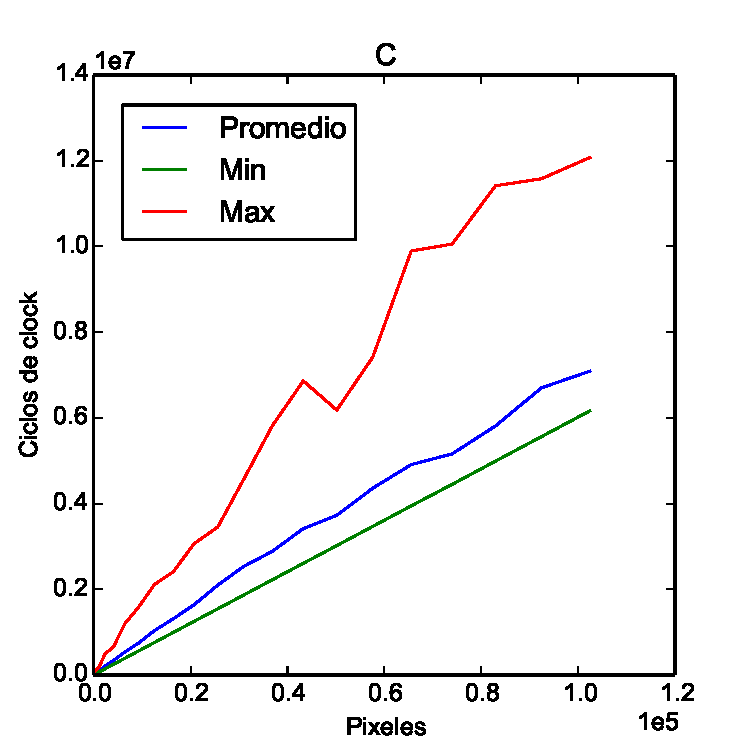
\includegraphics[scale=0.45]{images/c_merge}
	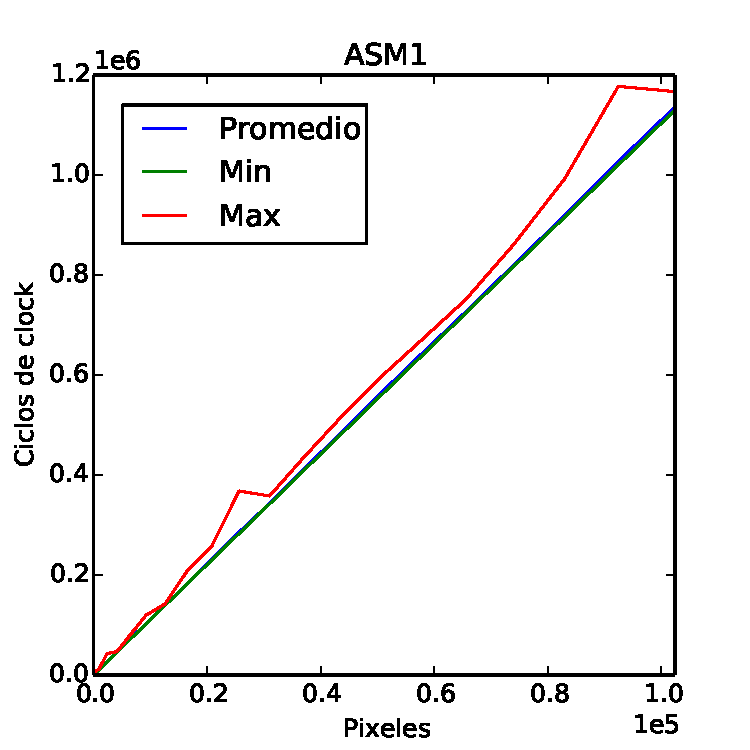
\includegraphics[scale=0.45]{images/asm1_merge}
	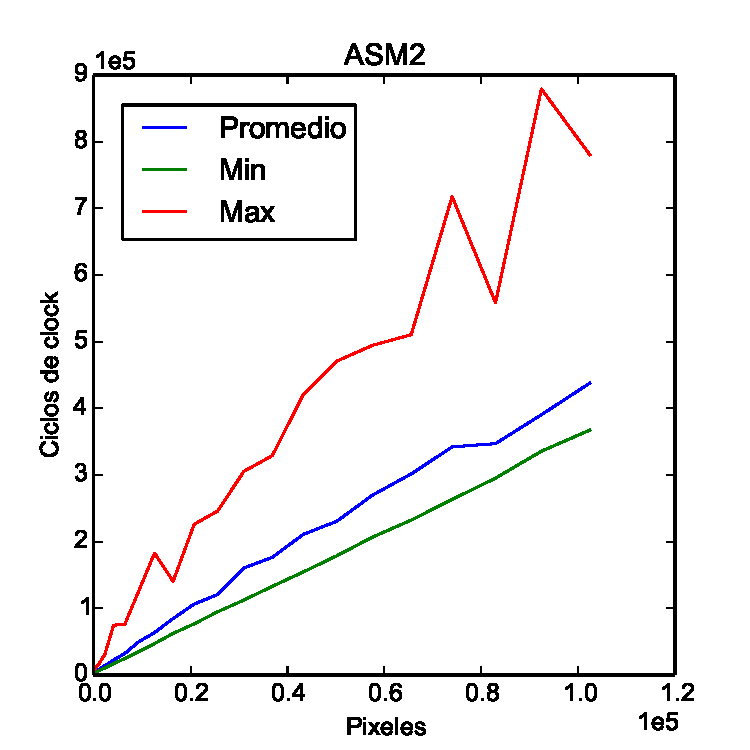
\includegraphics[scale=0.45]{images/asm2_merge}
\end{figure}

Tambien graficamos los 3 promedios en un grafico para ver cual de ellos es el mas rapido en general. Y para ver mejor la diferencia entre ASM1 y ASM2 los graficamos aparte.

\begin{figure}[h!]
	\centering
	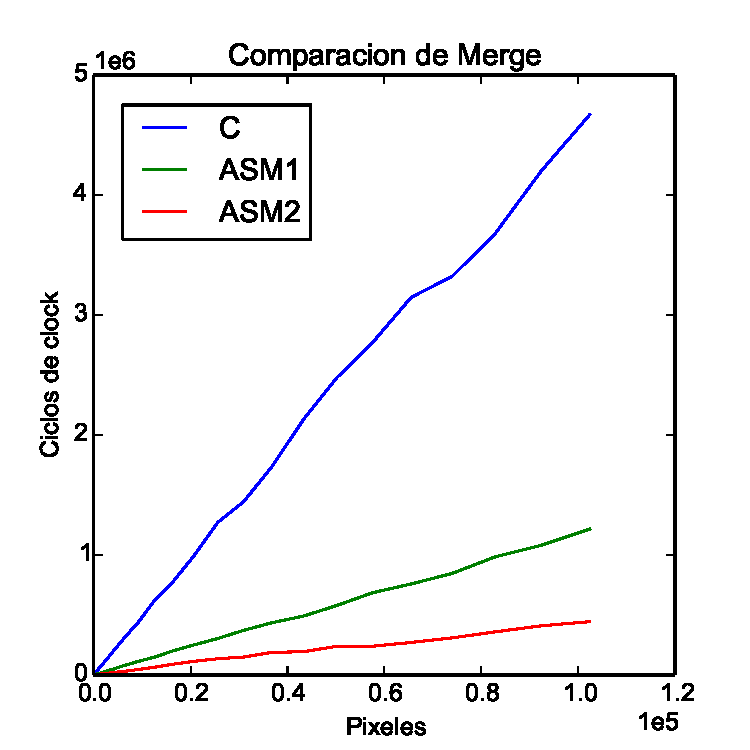
\includegraphics[scale=0.5]{images/c_asm1_asm2_merge_comp}
	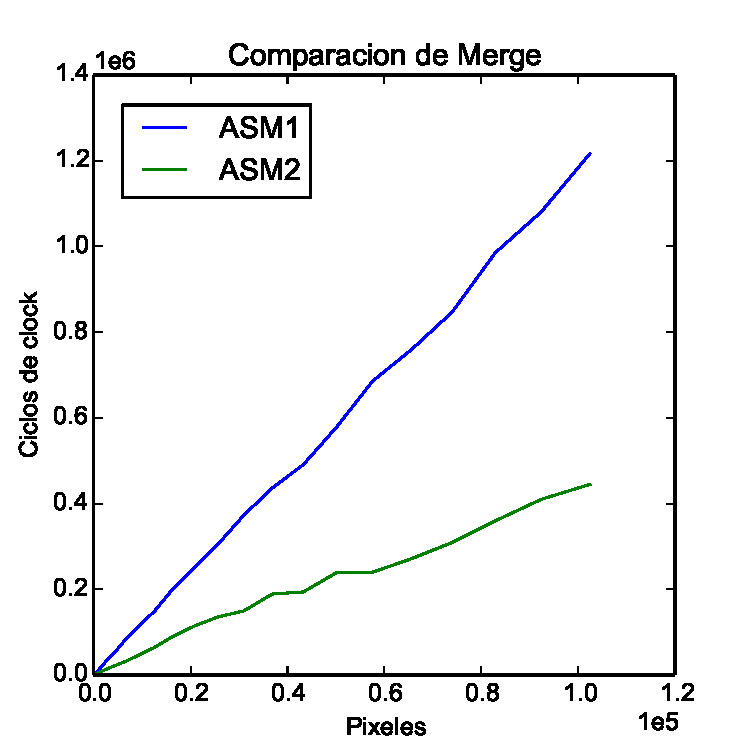
\includegraphics[scale=0.5]{images/asm1_asm2_merge_comp}
\end{figure}
\newpage

Tambien queremos ver que la imagen no modifique el tiempo de ejecucion, tanto el codigo de C como el de ASM no poseen ningun salto condicional que depende de el valor de los pixeles.

\begin{figure}[h!]
	\centering
	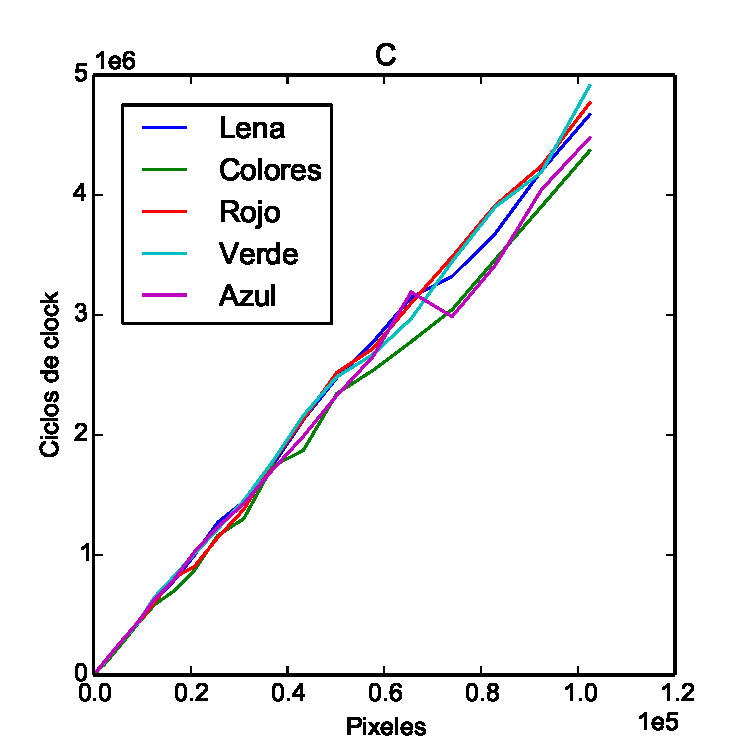
\includegraphics[scale=0.45]{images/c_merge_lena_colors}
	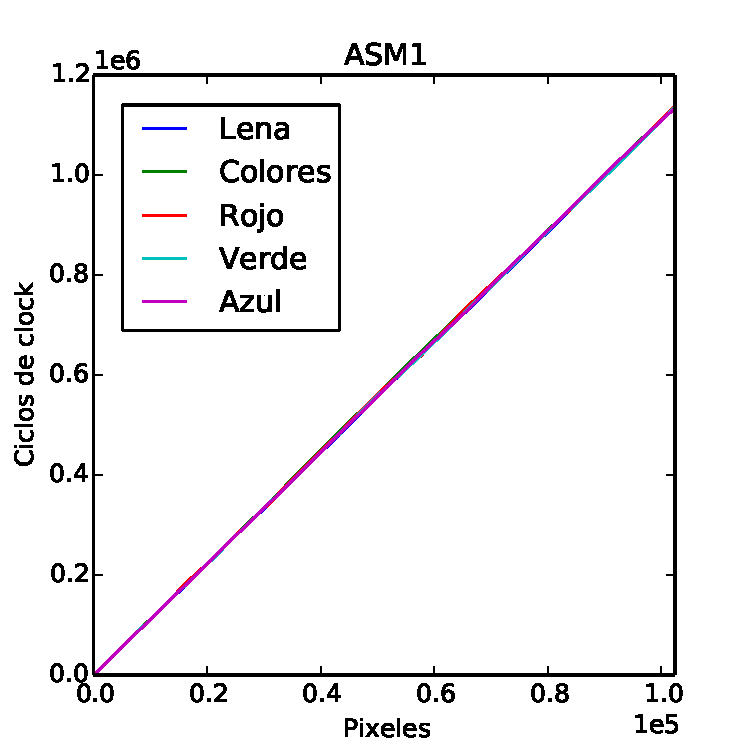
\includegraphics[scale=0.45]{images/asm1_merge_lena_colors}
	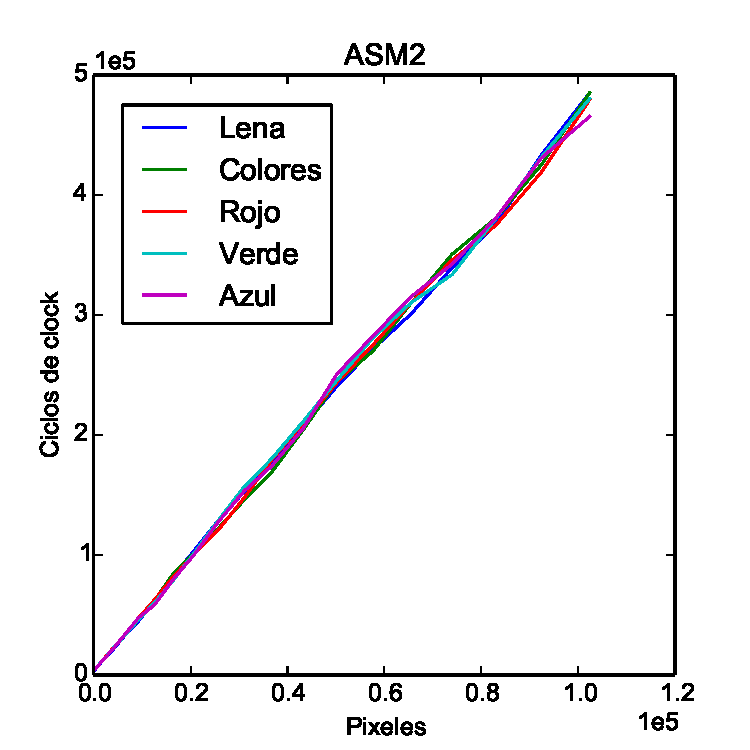
\includegraphics[scale=0.45]{images/asm2_merge_lena_colors}
\end{figure}

\subsection{Conclusion}

Al igual que en el primer filtro, las implementacion de $Assembler$ terminaron siendo mas veloces que la de $C$. La consistencia de los resultados tambien nos lleva a concluir que el costo en tiempo de hacer las conversiones en la primer implementacion es considerable, ya que la segunda version, al estar realizada sobre enteros minimizando las operaciones de punto flotante, tardo considerablemente menos.